\documentclass{beamer}

\usepackage{amsmath}
\usepackage{amssymb}
\usepackage{cancel}
\usepackage{graphicx}
\usepackage{hyperref}
\graphicspath{ {./img/} }

\usetheme{Warsaw}
\setbeamertemplate{headline}{}
\setbeamertemplate{page number in head/foot}[totalframenumber]

%Information to be included in the title page:
\title{Modelling Root Growth with Hormone Gradients}
\author{Riley Wheadon}
\institute{University of British Columbia}
\date{May 16th, 2024}

\begin{document}

\frame{\titlepage}

\begin{frame}
\frametitle{Table of Contents}
\tableofcontents
\end{frame}

\section{Extracellular Systems}

\subsection{Root Structure}

\begin{frame}
\frametitle{Structure}

The root is composed of \emph{three distinct regions}:
\begin{itemize}
	\item \textbf{Differentiation Zone} (DZ): Cells stop growing and develop specialized function. Differentiation occurs when cells reach a certain size (Pavelescu et al., 2018).
	\item \textbf{Elongation Zone} (EZ): Rapid growth, minimal division.
	\item \textbf{Meristematic Zone} (MZ): Rapid division, minimal growth.
\end{itemize}

\end{frame}

\subsection{Hormones}

\begin{frame}
\frametitle{Brassinosteroid and Auxin}

\textbf{Brassinosteroid} (BR) induces cell \emph{growth}. Higher levels of BR are found far from the root tip in the elongation zone.

\bigskip

\textbf{Auxin} induces cell \emph{division}. Higher levels of auxin are found near the root tip in the meristematic zone.

\end{frame}

\subsection{Model}

\begin{frame}
\frametitle{Modelling BR and Auxin}

We model BR and Auxin using a \textbf{Logistic Function}:
$$\begin{aligned}
	\text{B}(x) &= \frac{1}{1 + e^{a(x - m)}} \\[5pt]
	\text{A}(x) &= 1 - \text{B}(x)
\end{aligned}$$

\begin{itemize}

	\item $x$ denotes the distance from the top of the root.
	\item $a$ sets the size of the transition region.
	\item $m$ sets the boundary between the EZ and MZ.
\end{itemize}

\end{frame}

\begin{frame}
\frametitle{Discretization}

We built the model by considering discrete time intervals $\Delta t$. The growth of a cell over $\Delta t$ is 
$$G(x, \Delta t) = B(x) \cdot \Delta t  $$

The probability of a cell dividing in $\Delta t$ is
$$P(x, \Delta t) = A(x) \cdot \Delta t$$

To check for division, we generate a random $p \in [0, 1]$. If $p < P(x, \Delta t)$, the cell splits into two cells of half the size.

\bigskip


\end{frame}

\begin{frame}
\frametitle{Model}

\textcolor{blue}{\href{https://github.com/rileywheadon/plant-growth/blob/master/presentation/model1.gif}{Link}}

\end{frame}

\section{Intracellular Systems}

\subsection{Microtubule Organization}

\begin{frame}
\frametitle{Microtubule Organization}

\textbf{Microtubules} (MTs) are a thread-like polymer that supports the cytoskeleton of a cell. \textbf{CLASP} controls how MTs are arranged.

\begin{figure}
	\centering
	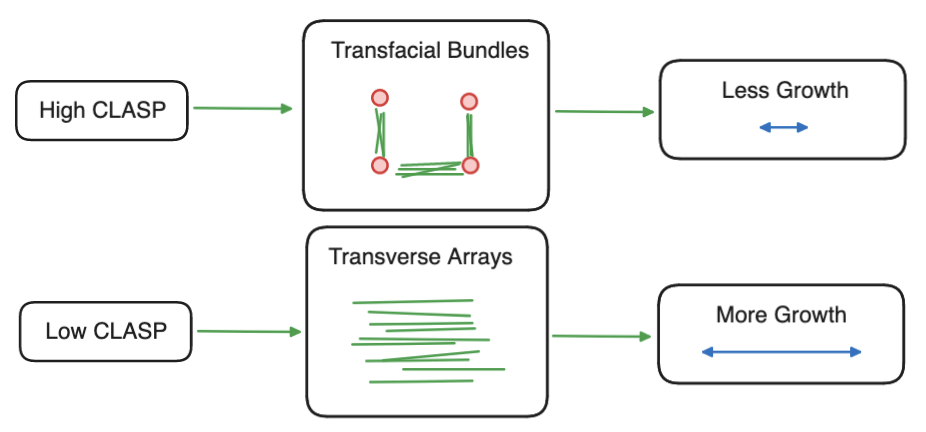
\includegraphics[scale = 0.5]{fig1.png}
\end{figure}

* This is a simplification of agent-based simulations.

\end{frame}


\begin{frame}
\frametitle{BR, MTs, and CLASP}
\textbf{BR} binds to receptors on the membrane. When \textbf{CLASP} is high, the cell begins to produce new receptors.

\begin{figure}
	\centering
	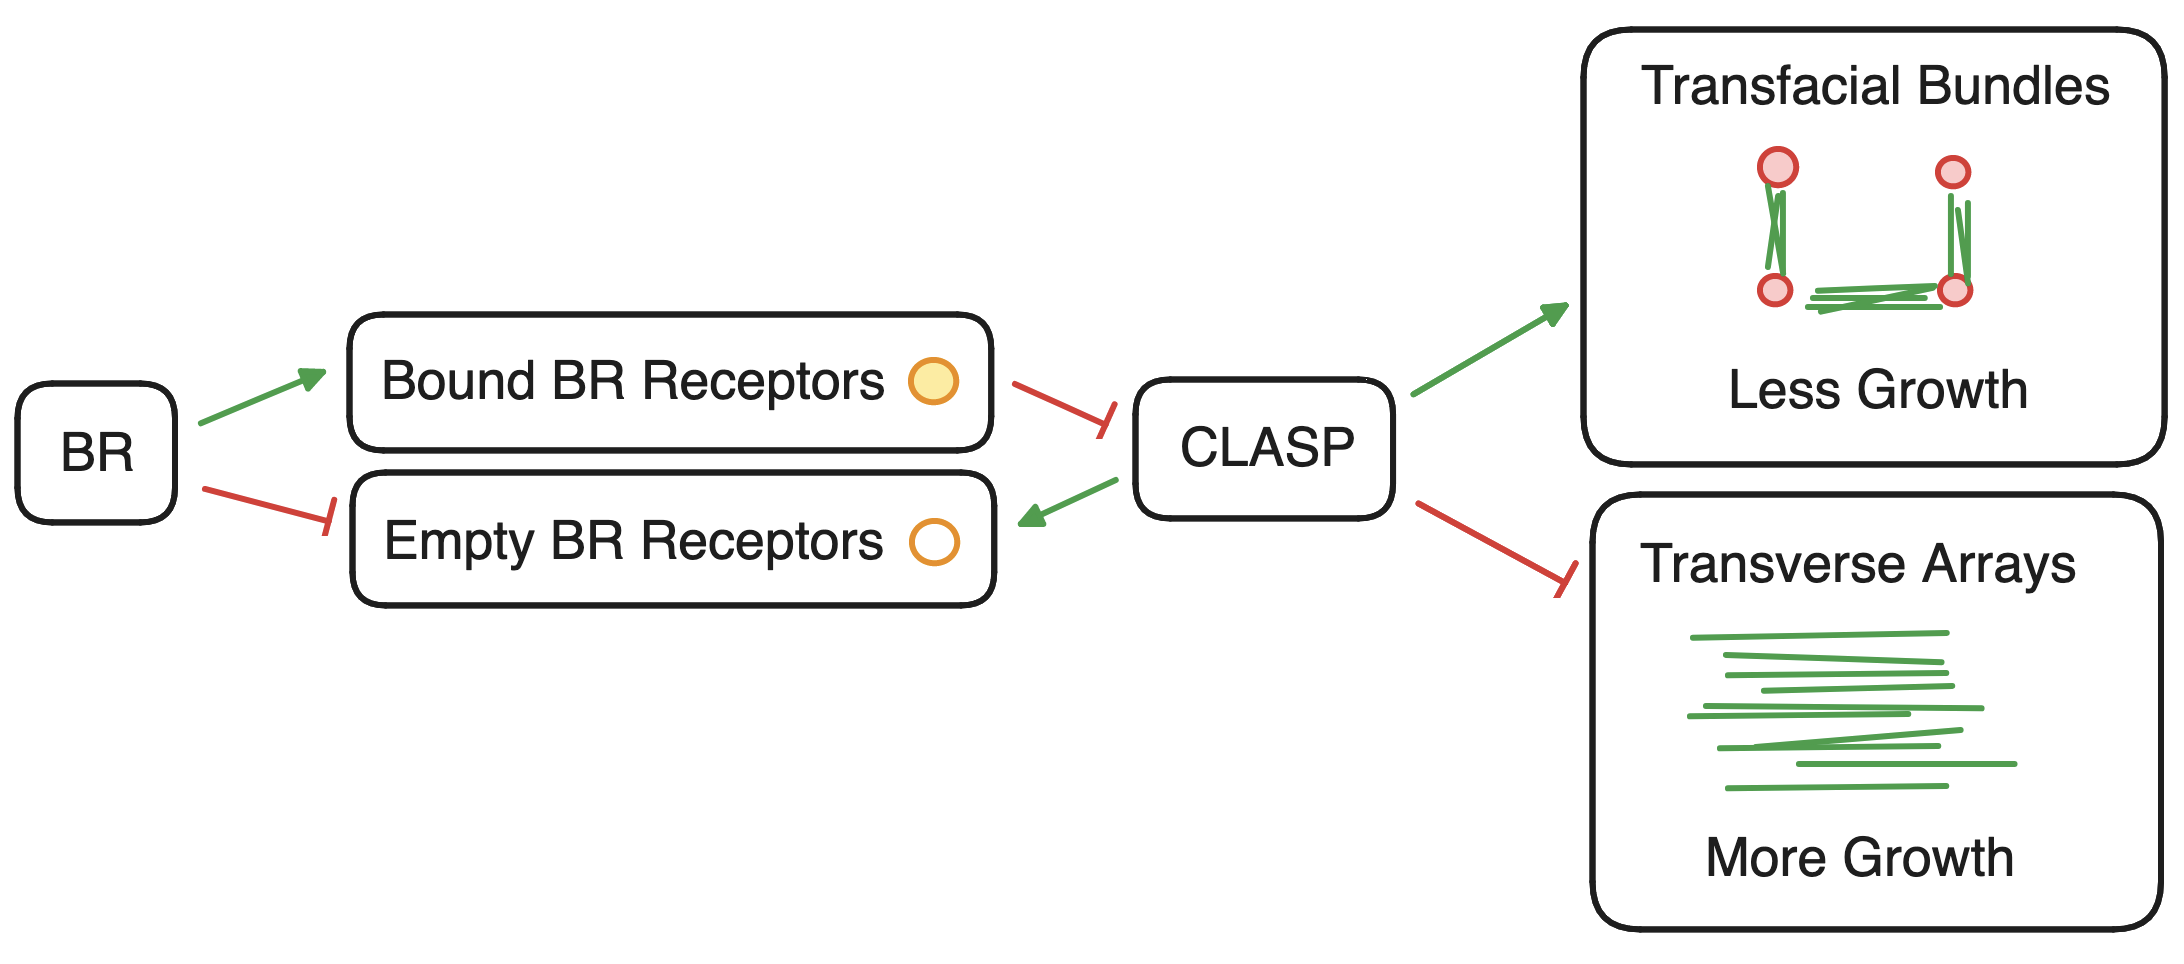
\includegraphics[scale = 0.27]{fig2.png}
\end{figure}

Our goal is to find the growth $(\phi)$ as a function of BR $(B)$. 

\end{frame}



\subsection{Model} 

\begin{frame}
\frametitle{Representing MTs with DEs}

\begin{figure}
	\centering
	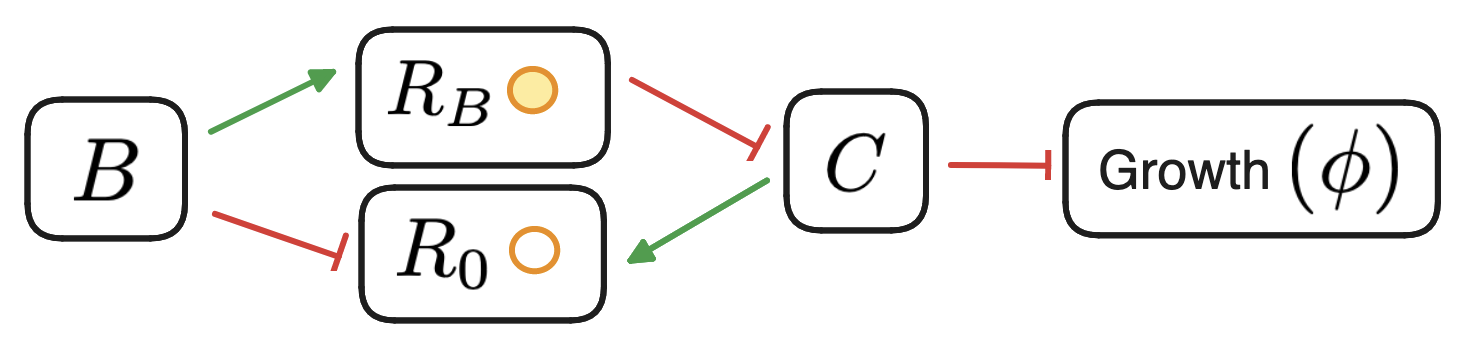
\includegraphics[scale = 0.3]{fig3.png}
\end{figure}

We used a system of differential equations to model the relationship between BR $(B)$, CLASP $(C)$, and receptors $(R_{0}, R_{B})$.
$$
\begin{cases}
C' = s - t(1 + uR_{B})C \\[5pt]
R_{0}' = v(1 + wC) - k_{\text{in}}^{ 0 }R_{0} - k_{\text{on}}BR_{0} + k_{\text{off}}R_{B} \\[5pt]
R_{B}' = k_{\text{on}}BR_{0} - k_{\text{in}}^{ B }R_{B} - k_{\text{off}}R_{B}
\end{cases}
$$
\end{frame}

\begin{frame}
\frametitle{Finding $\phi$}


Then, we represent the organization of the MTs as $\phi(B)$. This function is a simplification of work from Ambrose et al., 2011.
$$\phi(B) = \frac{C_{m}^{n}}{C_{m}^{n} + C(B)^{n}}$$

\begin{itemize}
	\item $\phi = 0$ represents high levels of TFBs (low growth).
	\item $\phi = 1$ represents transverse arrays (high growth).
\end{itemize}

\bigskip

We are still missing $C(B)$, but we have a trick!

\end{frame}

\begin{frame}
\frametitle{Time Scale Analysis}
We assume that extracellular processes take place on a much longer time scale than intracellular ones. This means each cell will quickly settle into a steady state, so

$$\begin{cases}
C' = 0 \\[5pt] R_{0}' = 0 \\[5pt] R_{B}' = 0
\end{cases}$$


\bigskip

Here is the \textcolor{blue}{\href{https://www.desmos.com/calculator/vcrxd7n1ju}{steady state solution}}. Now we have $\phi(B)$!

\end{frame}


\begin{frame}
\frametitle{Model}

\textcolor{blue}{\href{https://github.com/rileywheadon/plant-growth/blob/master/presentation/model2.gif}{Link}}

\end{frame}

\end{document}

